\section{Shared memory parallelisation}
\label{section:shared-memory}

We introduce three levels of shared memory parallelisation. On the highest level, we exploit the cell level decomposition and assign work within each cell to cores. Within the cell we assign work per particle pair  to an inner fork-level of threads. Lastly within each particle pair the innermost level of parallelisation is utilised to exploit mesh level parallelisation by the contact solver.

Three levels of multicore parallelisation:\\

a) cell level cell-to-cell thread units\\

b) cell vertex level particle-to-particle thread units\\

c) particle level mesh-to-mesh thread units\\

%describe the setup
We utilise particles approximated by a random spherical point cloud, arbitrary particle surfaces are generated with the Delauny triangulation algorithm. The algorithm is scaled in three respects; number of non-spherical particles, irregularity of particle radius size, and mesh size. Respectively, we provide three parameters in the creation of the simulation domain. $Rmin$, $Rmax$ parameter for max and min radius of particles, $m$ for mesh density, $p$ for number of particles in the domain. These allow observation of the interplay between performance and particle geometry and dynamics within a grid in a modern NUMA architecture. For scaling measuring we use the hybrid and the brute force solvers.

%Initial conditions
For the experiment the initial space configuration of the particles in respect to the grid is homogeneous and aligned per cell. Initial conditions for the particle dynamics are governed by the force of gravity only. The termination condition is a finite number of steps where the majority granulates of the experiment are rest and in contact position on a floor, this step phase is known a priori. We utilise regular grid and reluctant-adaptive grids for space decomposition and adaptivity. 

\begin{figure}[htb]
  \begin{center}
    \includegraphics[width=0.8\textwidth]{experiments/omp/omp_mesh_regular.png}
  \end{center}
  \caption{Regular grid drop test shared memory scaling of 729 particles, 22540 triangle elements.}
  \label{figure:omp_regular_triangle_20}
\end{figure}

\begin{figure}[htb]
  \begin{center}
    \includegraphics[width=0.8\textwidth]{experiments/omp/omp_mesh_reluctant.png}
  \end{center}
  \caption{Regular grid drop test shared memory scaling of 729 particles, 22540 triangle elements.}
  \label{figure:omp_reluctant_triangle_20}
\end{figure}

%I THINK I SHOULD MERGE THE ABOVE TWO PLOTS INTO ONE

Starting from the innermost level of parallelism, the tessellation-level experiment with a regular grid (figure \ref{omp_regular_triangle_20}) on a NUMA ivy bridge system scales up to the single eight-core die. As we increase the size of the problem using the m parameter (figure \ref{omp_regular_triangle_200}) we observe that computation to memory bandwidth is no longer sustainable over multiple cores. 

Similarly for a small enough sized $m$ (figure \ref{omp_reluctant_triangle_20}) adaptivity doesn't pay off as multi-threading scheduling, initialisation, adaptivity and communication overhead takes over computation. Contrary to regular grid, adaptivity allows up to scale on bigger problems (figure \ref{omp_reluctant_triangle_200}) as long as shared memory and computation to memory bandwidth overhead is not a bottleneck. In both cases for the brute force solver it did not scale pass the second die interconnect.



In the innermost level of parallesation we are experimenting with several solver methods to resolve contact points. At this level computation is parallelised upon triangle pairs and triangle batches and assigned to threads statically. 
From the performance measurements in Figure \ref{figure:triangle_omp} it is observed that Hybrid-on-triangle-pairs scales but it is slowest method to solution per timestep. 

\begin{figure}[htb]
  \begin{center}
    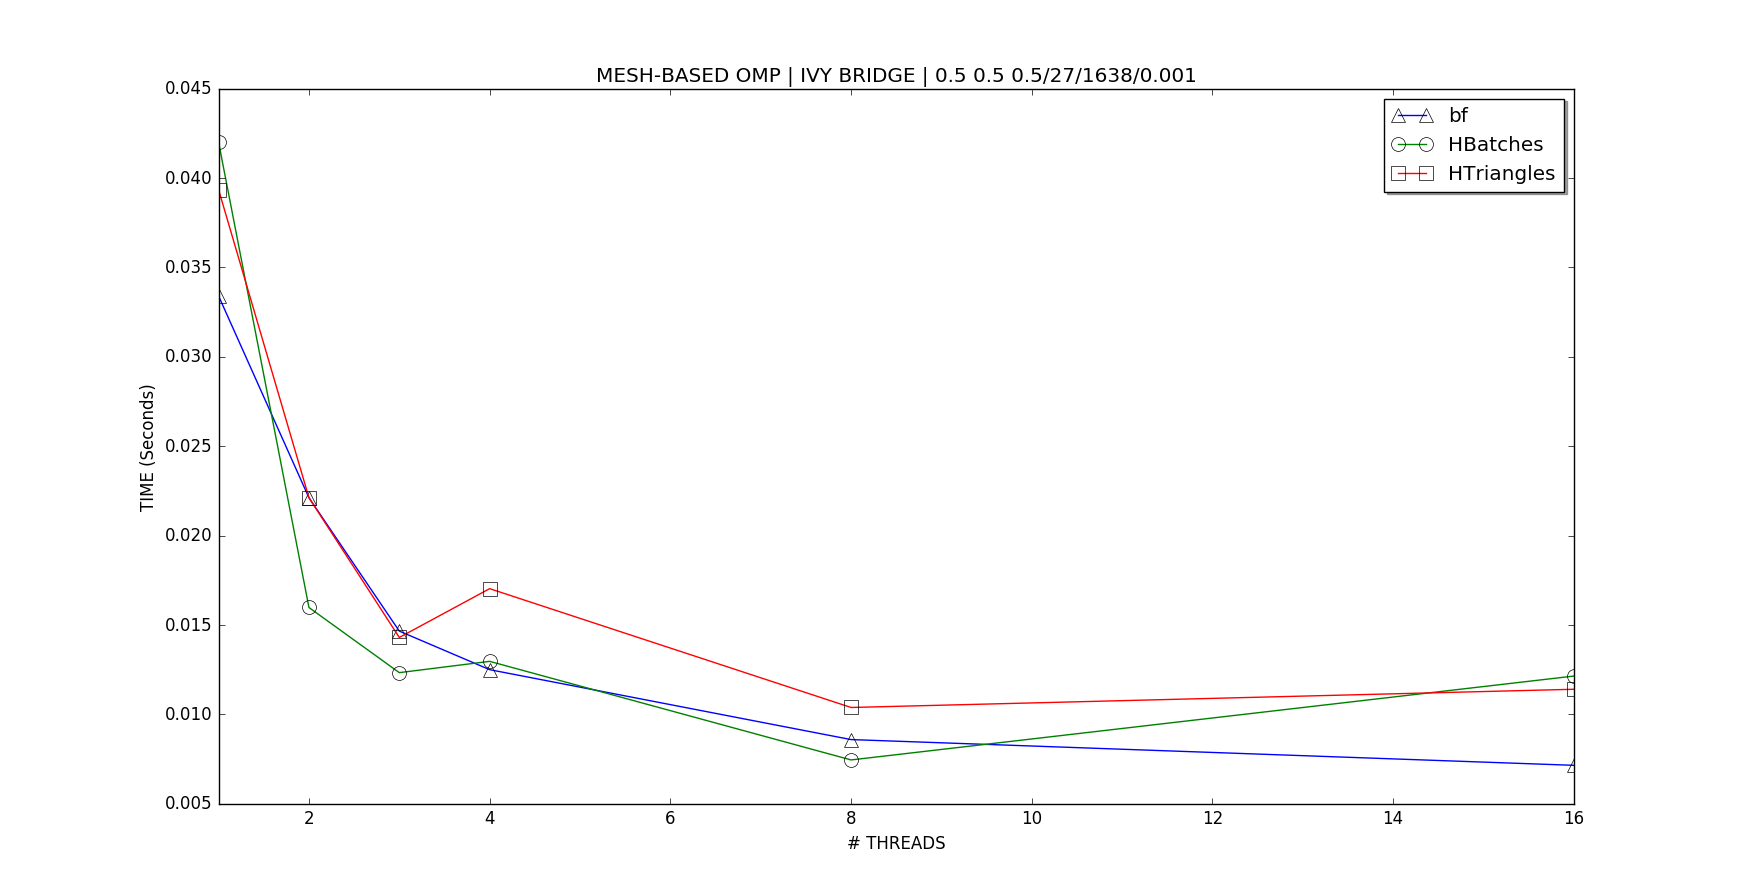
\includegraphics[width=0.8\textwidth]{experiments/random/omp/triangle_based_x0.png}
  \end{center}
  \caption{Triangle based shared memory parallelism using openMP running brute force (bf), hybrid-on-batches (HBatches) and hybrid-on-triangle-pairs (HTriangles) methods.}
  \label{figure:triangle_omp}
\end{figure}

\begin{figure}[htb]
  \begin{center}
    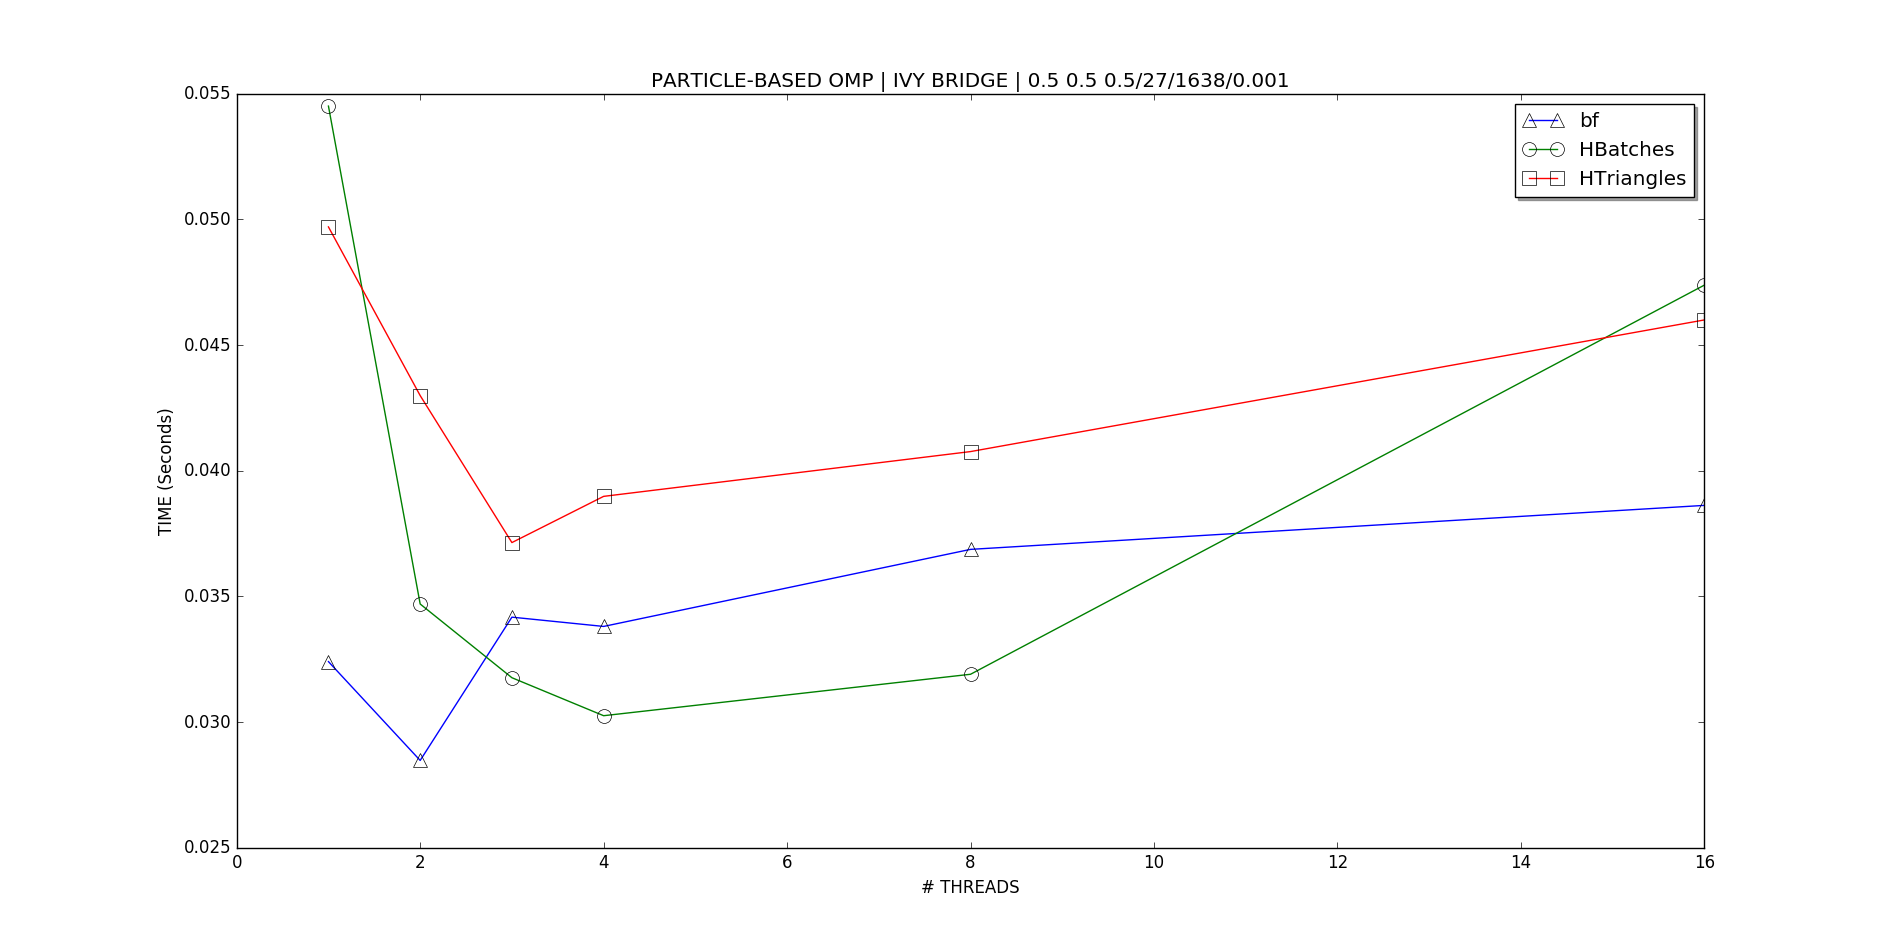
\includegraphics[width=0.8\textwidth]{experiments/random/omp/particle_based_x0.png}
  \end{center}
  \caption{Particle based shared memory parallelism using openMP running brute force (bf), hybrid-on-batches (HBatches) and hybrid-on-triangle-pairs (HTriangles) methods.}
  \label{figure:particle_omp}
\end{figure}

The alternative method of parallelisation is based on whole particle pairs. Thread subscription is performed during the outer sweeping of particles where pairs-of-particles per grid-vertex are computed in parallel on each vertex visit. In Figure \ref{figure:particle_omp} we see that again hybrid-on-triangle-pairs is performing worst and hybrid-on-batches to scale better. Brute force does not scale as well as hybrid-on-batches but has faster time to solution on low number of threads.

\begin{figure}[htb]
  \begin{center}
    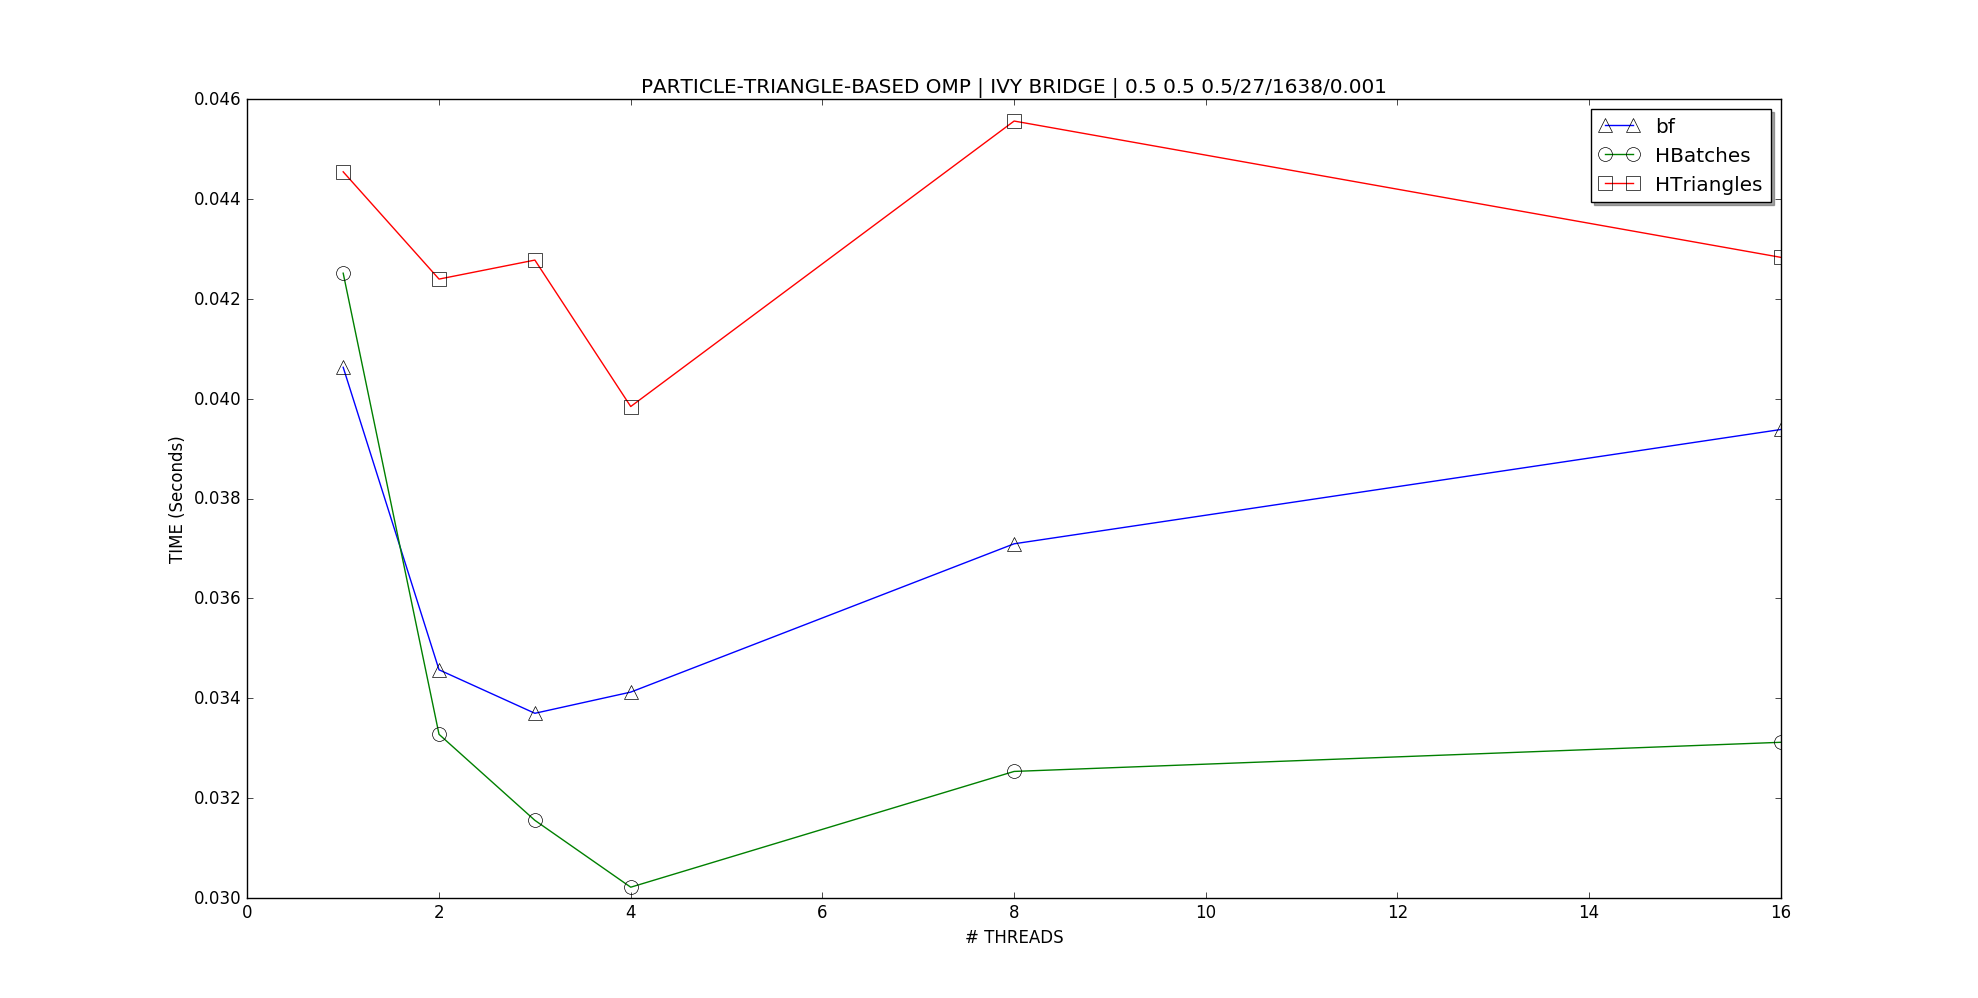
\includegraphics[width=1\textwidth]{experiments/random/omp/particle_triangle_based_x0.png}
  \end{center}
  \caption{Particle and Triangle based nested shared memory parallelism using openMP running brute force (bf), hybrid-on-batches (HBatches) and hybrid-on-triangle-pairs (HTriangles) methods.}
  \label{figure:particletriangle_omp}
\end{figure}

Particle and Triangle parallelism nests both particle and triangle shared memory threads. The runtime to solution is slightly slower than particle-based parallelism due to the thread/openMP overhead. Nevertheless it has an impact on brute-force method as it scales smoother than particle-based only parallelism due to overhead. In this case hybrid-on-batches is also the fastest while the hybrid-on-triangle-pairs the slowest. 

\clearpage

\begin{figure}[htb]
  \begin{center}
    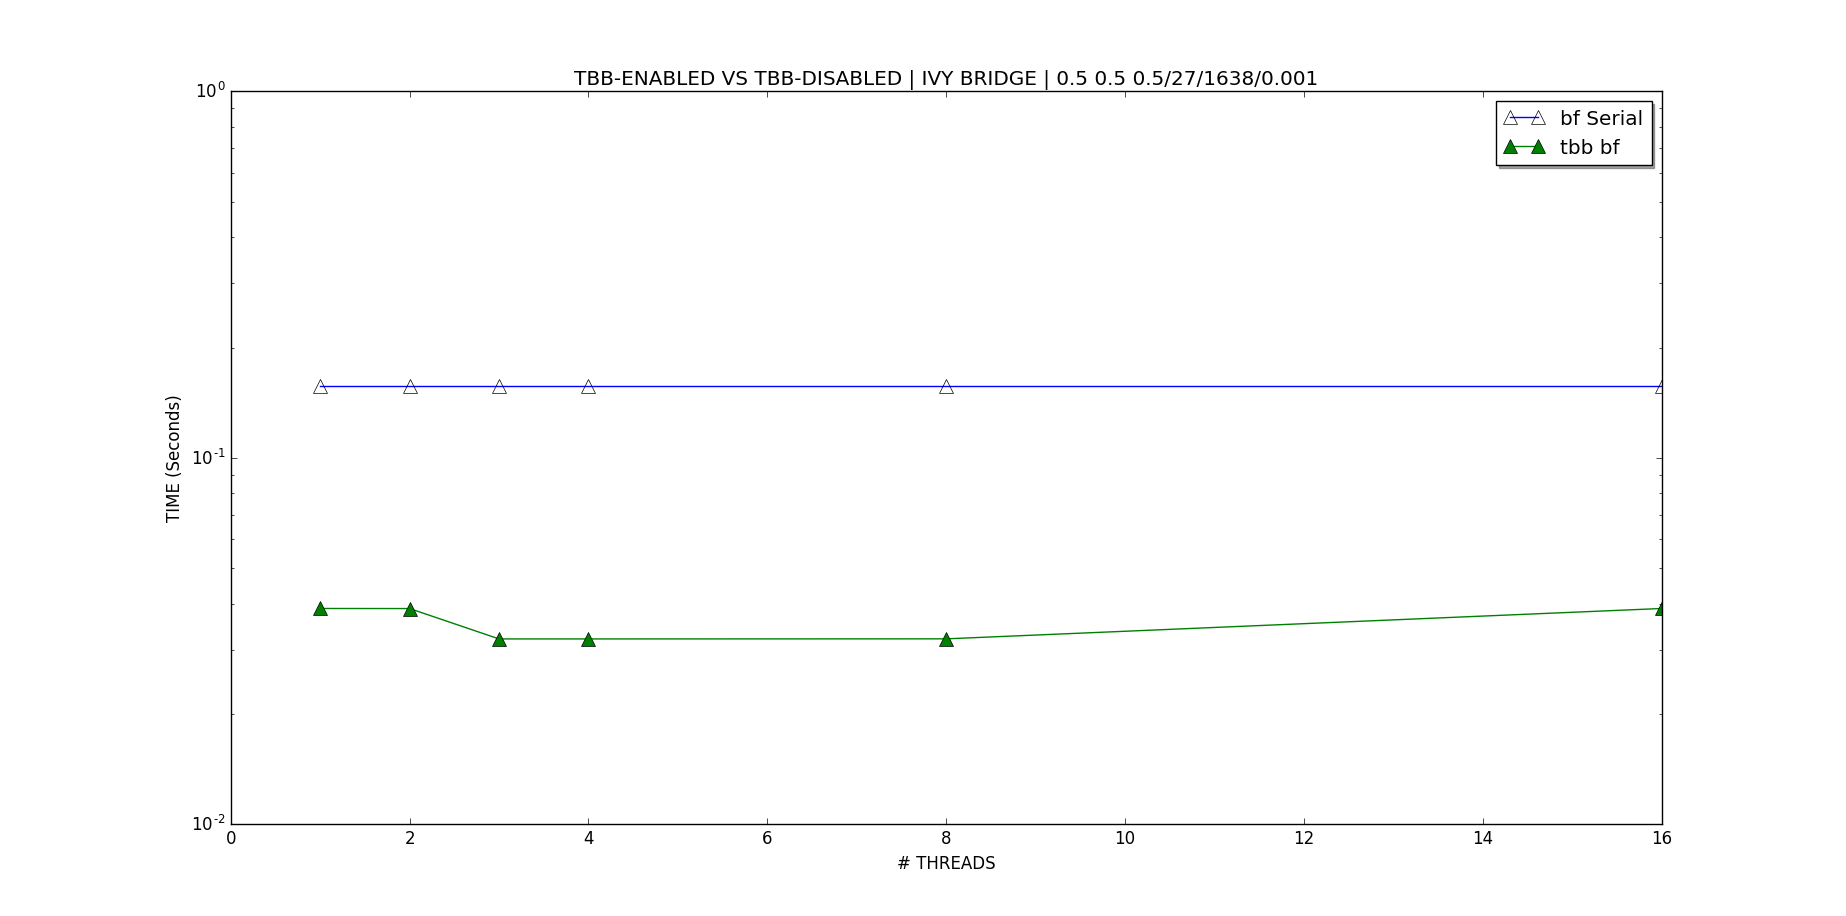
\includegraphics[width=1\textwidth]{experiments/random/omp/tbb_vs_serial.png}
  \end{center}
  \caption{Cell based parallelism on Peano compared to serial runs using Intel TBB}
  \label{figure:tbb_vs_serial}
\end{figure}

Another aspect of shared memory performance is thread scheduling and balancing implications.
The non-deterministic nature and error-prone distribution of triangles of the hybrid algorithm as discussed in Chapter {-hybrid chapter-} would suggest that alternative scheduling would pay off. But for our experiments dynamic and guided thread scheduling didn't not have a performance improvement on our tests but they rather create an scheduling overhead instead. That is partly due to the distribution of error in the triangle pairs and due to the granularity of our batches. Insignificant improvements were shown to our worst hybrid-on-triangle-pair method when using dynamic scheduling with OpenMP on the ivy bridge machine.    

At the highest level of shared memory parallelism is the grid cell-based multicore processing. It is based on the peano-framework that is using Intel TBBs to assign cells on threads. This has significant impact on the overall runtime performance in Figure \ref{figure:tbb_vs_serial} it is compared with plain serial execution. Number of threads on the x axis refer to TBB Cell-based threads, at the contact detection method level the computation is performed without shared memory parallelism but with vectorization enabled. For the specified experiment in Figure {} we observe no cell-based thread scaling but only reduction of time to solution. But when we increase the problem size further (figure \ref{figure:tbb_scaling}) we see that cell-based parallelism scales and it enhances execution time. 

\begin{figure}[htb]
  \begin{center}
    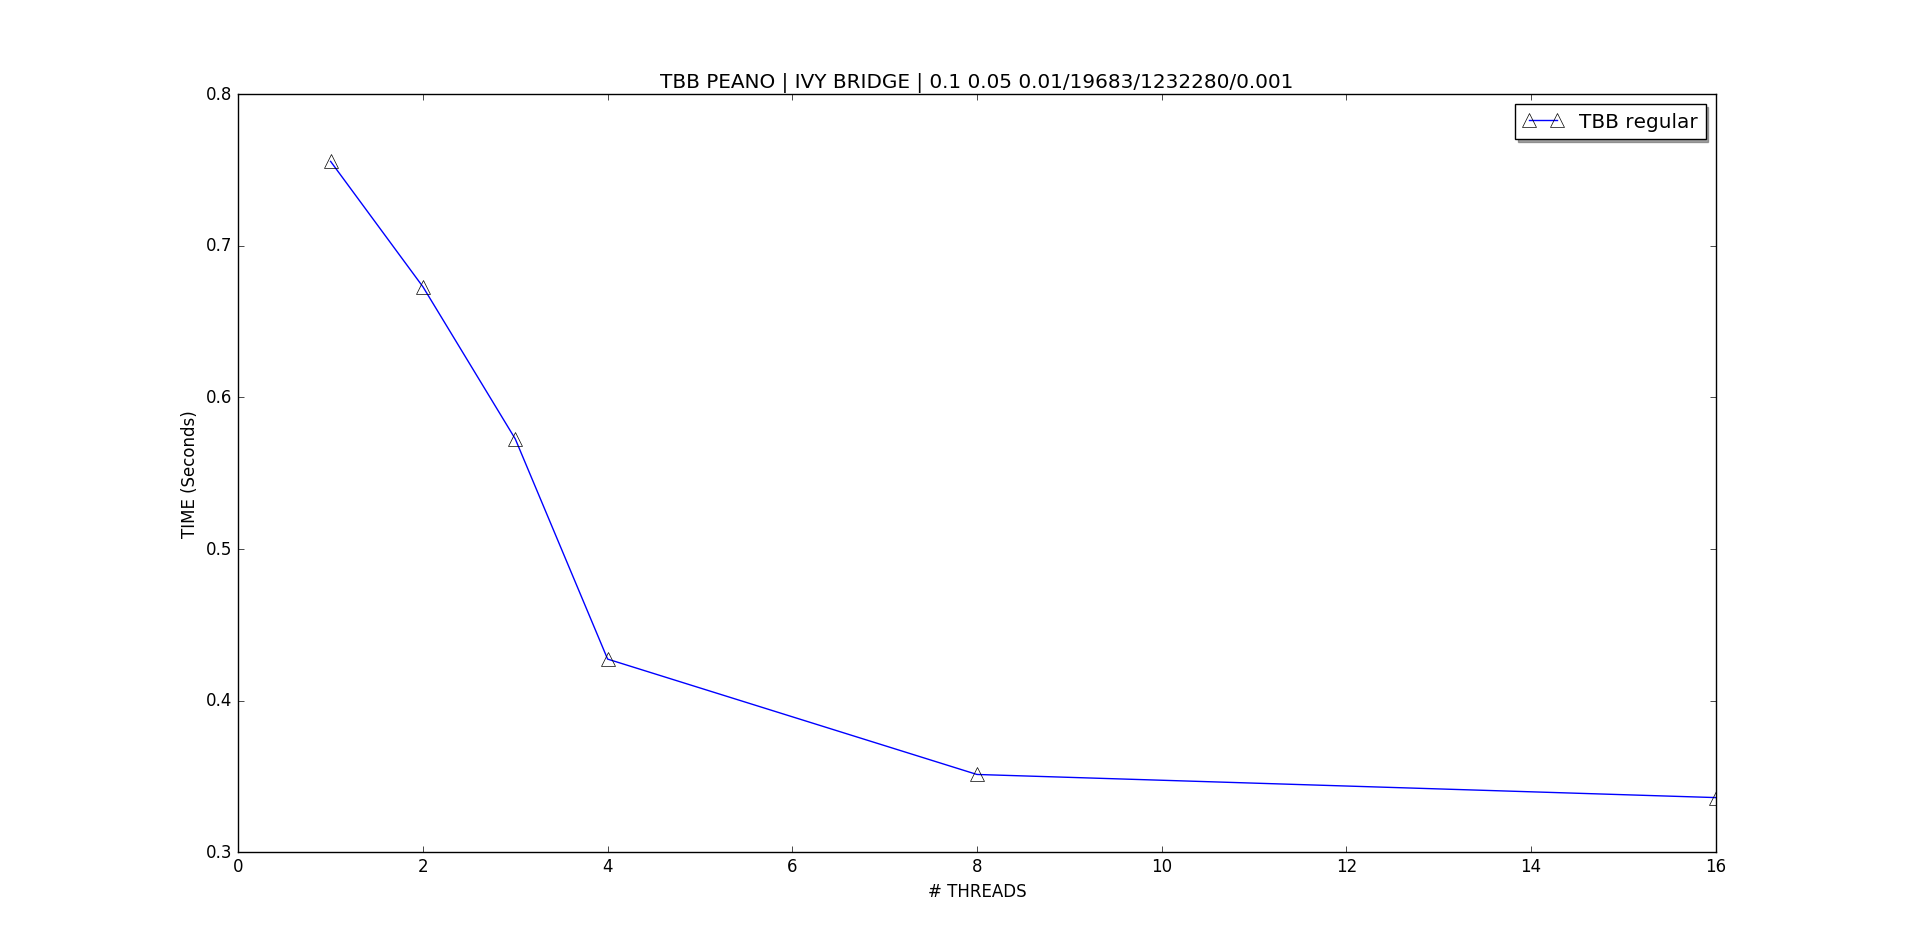
\includegraphics[width=0.8\textwidth]{experiments/random/omp/tbb_regular_x2.png}
  \end{center}
  \caption{Cell based parallelism on Peano compared to serial runs using Intel TBB}
  \label{figure:tbb_scaling}
\end{figure}

Overall shared memory parallelism on these three levels of parallelisation yield performance gain on manycore systems for our hybrid-on-batches method and in some cases brute force. For small problems triangle-based parallelism show good time to solution but for larger (**put plot) problem sizes particle-based parallelism pays off better. The finer/inner the thread forking the less significant scaling it is observed for larger problem sizes. For large problem sizes the combination of cell-based plus particle-based multi-core parallelism using hybrid-on-batches makes sense. Furthermore additional overall speedup can be gained if spheres are used as a filtering bounding box stage to our triangle-to-triangle contact detection.

\clearpage

